\namedchapter[Adam Zieliński]{Projekt oraz wykonanie płytki drukowanej}
Płytka drukowana jest to płytka wykonana z tworzywa izolacyjnego, na którą naniesione zostały komponenty elektroniczne połączone miedzianymi ścieżkami. W ogólności jest to sposób montażu układów elektronicznych zapewniający estetyczną oraz kompaktową strukturę. Znajdujące się na niej obwody są projektowane ściśle pod konstruowany układ.
\namedsection{Projekt}
Pierwszym etapem projektowania jest zaplanowanie rozmieszczenia komponentów na jej powierzchni. Dzięki temu można określić ostateczne wymiary przygotowywanej powierzchni, które w tym przypadku wynoszą 85x155 mm. Specjalnie stworzone do tego środowisko pozwala płynnie przejść z schematu ideowego do ,,widoku" płytki uwzględniając przy tym wstępne połączenia pomiędzy elementami. Bardzo dużo uwagi należy poświęcić sprawdzeniu oznaczeń obudów zastosowanych układów oraz ich rozmiary, gdyż może okazać się, że zakupiony układ ma inny, niżeli wcześniej założony, kształt. W momencie, gdy wszystkie części są poukładane możemy rozpocząć proces łączenia sugerowanych przez środowisko pinów. Poprowadzone ścieżki powinny mieć określoną grubość - w zależności od wartości płynących przez nią prądów. Docelowo linie zasilające powinny być najszersze - tutaj 2 mm. Mimo licznych prób nie udało się poprowadzić wszystkich ścieżek na jednej stronie laminatu. W związku z tym zaprojektowana została płytka dwustronna - czyli posiadająca ścieżki po obu stronach. Ścieżki połączone zostały przez tzw. przelotki, czyli niewielkie miedziane druty przechodzące przez laminat. Wszystkie wykorzystane elementy pozwalają na montaż przewlekany, przez co niezbędne jest wykonanie w płytce otworów przeznaczonych na wyprowadzenia elementów. Wyprowadzenia te zrealizowane są w formie drucików, które przewleka się przez otwory i lutuje do ścieżki. Rysunek \ref{plyta} przedstawia ostateczny projekt płytki drukowanej. Część A to warstwa dolna, do której przylutowane zostały komponenty, B - wierzchnia.
\newpage
   \begin{figure}[H]
    \begin{center}
      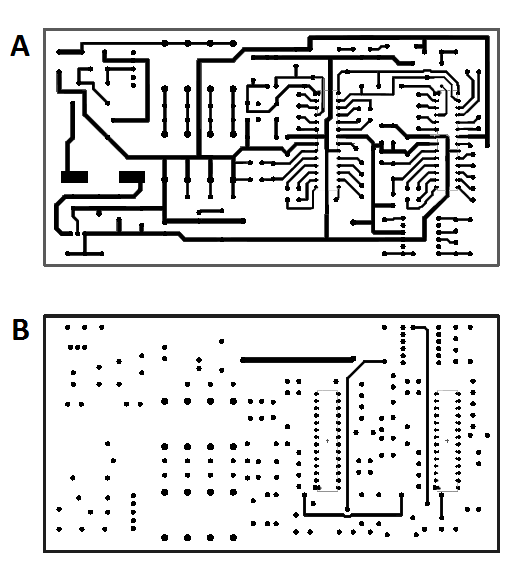
\includegraphics[scale=0.85]{imgs/plytka.png}
 	\caption[Projekt płytki drukowanej.]{\small{Rysunek przedstawia finalny projekt płytki drukowanej. Segment A przedstawia dolną jej dolną część - do której elementy są przylutowane, B - wierzchnią. }}
	\label{plyta}
    \end{center}
  \end{figure}   
\namedsection{Wykonanie}
Wykonanie płytki drukowanej należy rozpocząć od przeniesienie gotowego projektu bezpośrednio na powierzchnię pokrytą miedzią. Do tego celu wykorzystany został papier kredowy oraz drukarka laserowa. Wspomniany papier jest bardzo śliski oraz bardzo słabo ,,łączy" się z tonerem. Dzięki temu wydrukowany na niej układ stosunkowo słabo przywiera do jej powierzchni - co umożliwia jego dalszy transfer. Odpowiednio skrojony fragment laminatu należy bardzo bardzo dokładnie odtłuścić, np. przy użyciu acetonu. Opcjonalnie można także jego powierzchnię nieco zmatować przy wykorzystaniu papieru ściernego o wysokiej granulacji. Kolejnym etapem jest odbicie projektu na laminacie. W związku z tym papier kredowy należy możliwie dokładnie umieścić na płytce drukiem do jej powierzchni oraz zgrzać np. żelazkiem. Toner w temperaturze około 200$^\circ$C topi się i ,,odrywa" od papieru przywierając do miedzianej warstwy. Następnie wystarczy delikatnie usunąć papier. Nadrukowane tonerem ścieżki pozostają na płytce. Pozostaje jedynie umieścić płytkę w wytrawiaczu - nadsiarczanie sodu. Jest to środek o silnych właściwościach utleniających. Jego wodny roztwór wchodzi z reakcję z niezakrytą tonerem miedzią, utlenia ją i rozpuszcza.  Poniżej (rys. \ref{trwa}) znajdują się zdjęcia przedstawiające laminat bezpośrednio przed (A) oraz po (B) trawieniu. Kąpiel w utleniaczu powinna trwać tak długo, do momentu aż miedź całkowicie nie zniknie.

   \begin{figure}[H]
    \begin{center}
      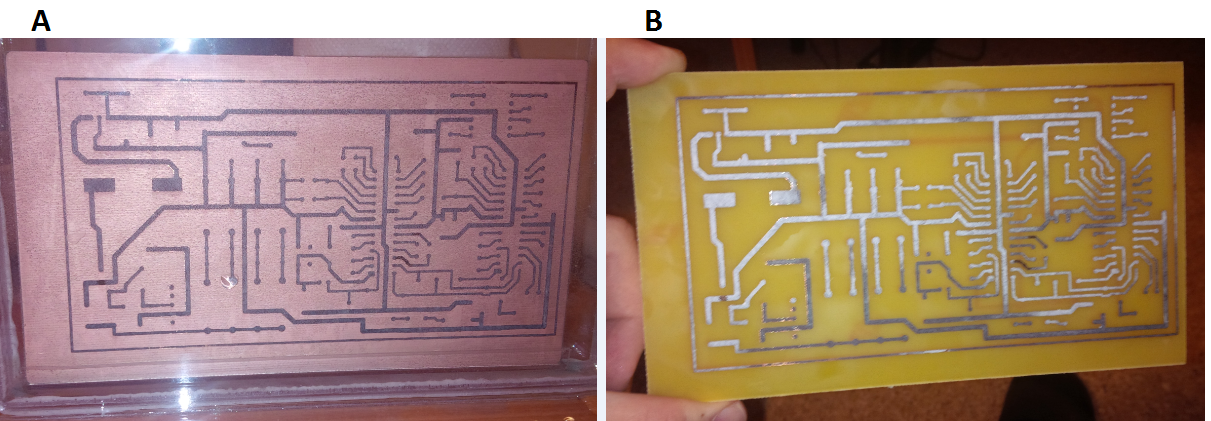
\includegraphics[scale=0.47]{imgs/plytka_trawienie.png}
 	\caption[Proces trawienia.]{\small{Zdjęcia przedstawiają pierwszy etap wykonywania płytki drukowanej. Fotografia A przedstawia laminat z przeniesionymi ścieżkami, umieszczony w wytrawiaczu. B - efekt wytrawienia.}}
	\label{trwa}
    \end{center}
  \end{figure}  
  
  Ostatnim etapem jest przylutowanie wszystkich komponentów. Efekt końcowy został przedstawiony na zdjęciach \ref{ost_ef}.
  
  \begin{figure}[H]
    \begin{center}
      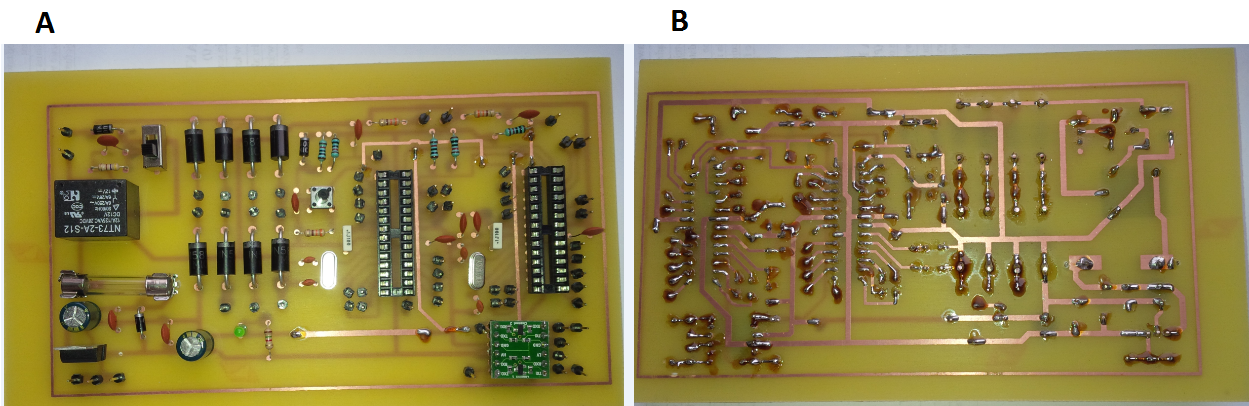
\includegraphics[scale=0.45]{imgs/efekt.png}
 	\caption[Wykonanie płytki drukowanej.]{\small{Zdjęcia przedstawiają kompletną, działająca płytkę drukowaną. Fotografia A przedstawia warstwę górną, B - warstwę dolną.}}
	\label{ost_ef}
    \end{center}
  \end{figure}  